% !TEX root = ../thesis.tex

\chapter{Background}
\label{ch:background}

In this chapter we describe existing technology and concepts that will be referred to throughout the thesis.

\section{GitHub}

QuickFeed already relies on GitHub to manage assignments and student code.
This section looks at certain GitHub features that we want QuickFeed to support.

\subsection{Issues}

GitHub issues is a useful feature for tracking, discussing and logging various issues/problems on a GitHub repository.
Any collaborator to a repository may open a GitHub issue, and describe any problem, idea or issue they have.
Other users may then contribute to the issue by commenting on it; thus easing the communication process within a project.
GitHub issues can therefore function as a discussion hub, and makes it especially useful for larger projects involving several people. 

\begin{figure}[ht]
    \centering
    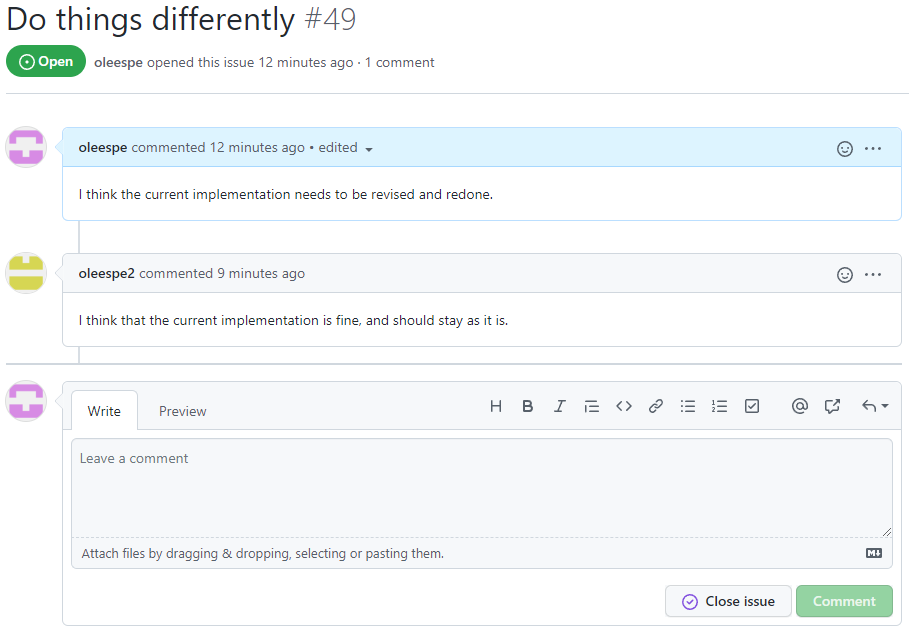
\includegraphics[width=\textwidth]{photos/github-issue.PNG}
    \caption{Example of a GitHub issue comment section}
    \label{fig:github-issue}
\end{figure}

\subsection{Pull Requests}

Pull requests are a desire to merge any feature branch, into the main branch of a git repository.
GitHub supports managing pull requests through its user interface, and allows any contributor to a repository to create a pull request.
Through the user interface, progress on a branch can be tracked, reviewed and commented on.
In this sense, GitHub pull requests function as a central hub for feature branches.

Code review is also a central part of the pull request process.
Any eligible user may review, comment on, and request changes to the source code of a given pull request.
The reviewer may also use reviews to approve a pull request for merging.

Pull requests can also be linked to issues.
Doing this will automatically associate any linked issue to the pull request, and cause them to close when the pull request closes.
A common workflow would be to create an issue, describing a problem, and then creating an associated pull request for this issue.

Through its features, GitHub pull requests provide an efficient and manageable way of implementing new features to any project.

\begin{figure}[ht]
    \centering
    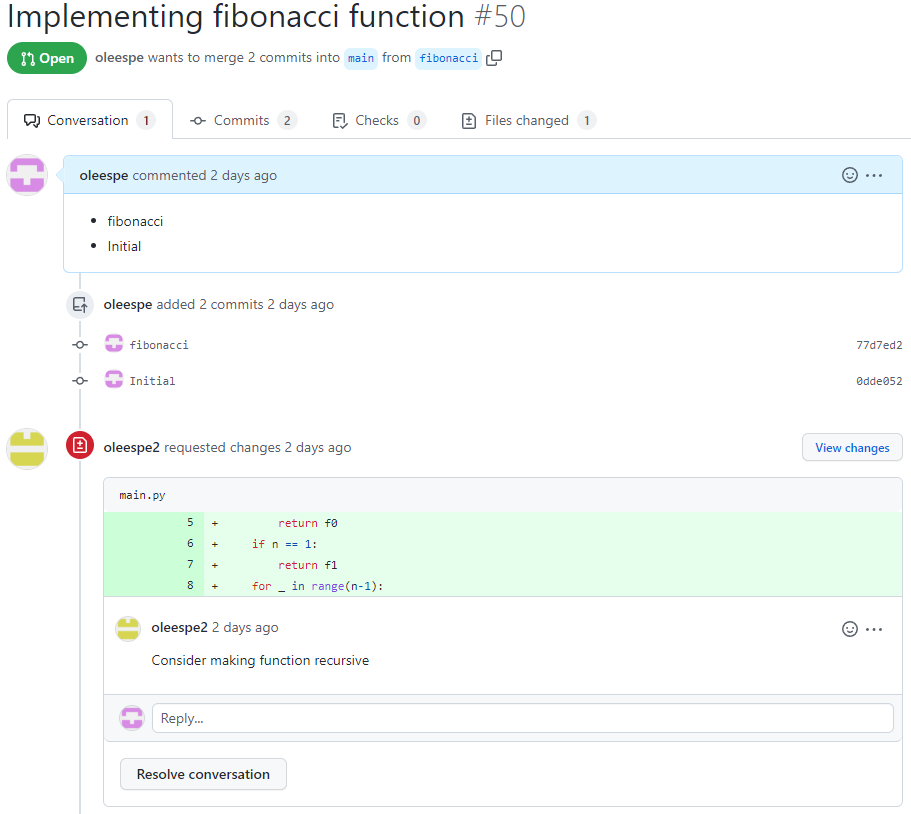
\includegraphics[width=\textwidth]{photos/pull-request.PNG}
    \caption{Example of a GitHub pull request}
    \label{fig:pull-request}
\end{figure}

\subsection{Workflows}

Maybe maybe

\section{QuickFeed}

QuickFeed provides two primary features.
A web interface that allows students to enroll in courses, create groups and receive feedback on their submissions.
And a backend that tests, scores and grades student submitted code.
The backend is primarily implemented with the Go programming language, while the frontend uses TypeScript and the React library.
For data storage, QuickFeed relies on an SqLite-database, managed using the the GORM library.

In this section we further describe some of QuickFeed's key concepts, as well as the technology it uses.

\subsection{Protocol Buffers}

Protocol buffers is a language-neutral mechanism for serializing structured data. % (ref: https://developers.google.com/protocol-buffers)
It is often abbreviated as protobuf, and is used to define messages in a \textit{.proto} file.
When the file is compiled, data structures and methods for the desired language are generated in a separate file.
QuickFeed uses protobuf to generate most of its data structures.
These are then stored in its internal database when necessary.

\begin{lstlisting}[caption={Assignment message}, label={code:Assignment}]
message Assignment {
    uint64 ID                       = 1;
    uint64 CourseID                 = 2;
    string name                     = 3;
    string scriptFile               = 4;
    string deadline                 = 5;
    bool autoApprove                = 6;
    uint32 order                    = 7;
    bool isGroupLab                 = 8;
    uint32 scoreLimit               = 9;
    uint32 reviewers                = 10;
    uint32 containerTimeout         = 11;
    repeated Submission submissions = 12;
    repeated GradingBenchmark gradingBenchmarks = 14;
}
\end{lstlisting}

Code \ref{code:Assignment} is an example of such a message.
It holds a reference to a single \textbf{Course} message and several \textbf{Submission} messages, as seen on Line 3 and 13 respectively.
When compiled, the resulting data structure is used by QuickFeed to represent assignments.

It should be noted that QuickFeed also uses all these messages in conjunction with gRPC to facilitate server-client communication.
This part is however not relevant for this project.

\subsection{QuickFeed Repository Structure}
\label{sec:quickfeed-repository-structure}

When a teacher creates a course in QuickFeed, a GitHub organization is created to represent it.
Within this organization, three initial repositories are created, as well as student repositories when students enroll.
They are all described as follows.

\textit{info}: This repository simply holds information about a course.
The repository is available to all students, and would typically work as a simple information hub.
It is created and managed by the teaching staff.

\textit{assignments}: The repository responsible for presenting the assignments to students.
Every assignment in a course is represented as a unique folder within this repository.
As teachers push new assignments to this repository, or update existing ones, students pull the changes to their own local git repositories.

\textit{tests}: Teachers use this repository to store both test code and files needed to facilitate automatic testing of student code.
It's folder structure should be one-to-one with \textit{assignments}, with every assignment being represented by a unique folder.
As students submit code for an assignment, QuickFeed tests it with all code from the folder representing that assignment.
In addition, the repository contains assignment specific \textit{assignment.yml} files, as well as a \textit{scripts} folder.
The \textit{scripts} folder is used to store a \textit{run.sh} file and a Dockerfile.

The \textit{assignment.yml} file is used by teachers to specify assignment specific settings.
As an example, it can contain information about the assignment deadline, whether it is manually graded, and more.

\begin{lstlisting}[caption={Example contents of an \textit{assignment.yml} file}, numbers=none]
assignmentid: 1
name: "lab1"
scriptfile: "run.sh"
deadline: "15-05-2022T16:00"
autoapprove: false
isgrouplab: true
\end{lstlisting}

The \textit{run.sh} file contains the script used by QuickFeed when testing student code.
As explained, it is contained within the \textit{scripts} folder, but can also be located within the specific assignments themselves.
When running tests on an assignment, QuickFeed will prioritize using any assignment specific script files.

Finally, the Dockerfile contained within \textit{scripts} is used to create a docker container.
Within this container, QuickFeed runs the appropriate script, derived from \textit{run.sh}.

\begin{figure}[ht]
    \centering
    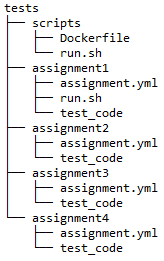
\includegraphics[scale=0.8]{photos/tests-repository-structure.PNG}
    \caption{Example of a tests repository folder structure}
    \label{fig:tests-repository-structure}
\end{figure}

Every time a teacher pushes to \textit{tests}, QuickFeed runs the function UpdateFromTestsRepo.
This function will parse an assignment's \textit{assignment.yml} file, and use its contents to create data objects defined by the \textbf{Assignment} message.
They are then used to create or update assignment database records.

Being a repository that is used and managed solely by the teaching staff, it follows that students do not have access to its contents.

Student repositories: There are two types of student repositories, user and group repositories.
A user in this case would simply be any student who has enrolled in the course.
Whereas a group is any number of students that are working together.
Naturally, student repositories are only accessible by the students associated with them, and the teaching staff.

Student repositories are named according to the following format: \textit{name-labs}.
For an enrolled student, \textit{name} would be their GitHub user name.
A group's \textit{name} however, would be defined by the group members themselves when they enroll the group.

These repositories are the ones students push their code to as they work on assignments.

\begin{figure}[ht]
    \centering
    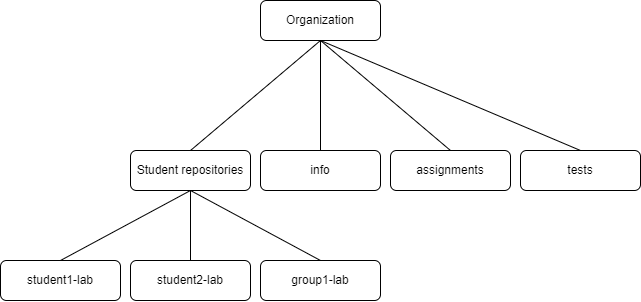
\includegraphics[width=\textwidth]{photos/qf-repository-structure.png}
    \caption{GitHub repository structure for a QuickFeed course}
    \label{fig:qf-repository-structure}
\end{figure}

\subsection{The Score Package}
\label{sec:the-score-package}

QuickFeed's score package allows for scoring student submitted code.
Every time a student pushes code to their repository, QuickFeed will run tests on the code, and generate a total score ranging from 0 to 100.
In this section we describe the parts of this package that are relevant for this thesis.

When teachers develop and push assignments to \textit{tests}, they also create test code that is meant to test student submitted code.
As part of the score package, teachers can specify for individual tests, what score they should give, and how that score is gained.
For example, a test can loop through several test conditions, and then decrement the score every time it fails.
These tests have to be explicitly added by teachers using either of the following methods: Add and AddSub.
Doing so, they are included in the pool of all tests that constitute an assignment.

Each individual score is defined by the protobuf message in Code \ref{code:Score}.
When QuickFeed is finished running all tests, a test results data object is extracted containing a list of all these scores.

\begin{lstlisting}[caption={Score message}, label={code:Score}]
message Score {
    uint64 ID =           1;
    uint64 SubmissionID = 2;
    string Secret =       3;
    string TestName =     4;
    int32 Score =         6;
    int32 MaxScore =      7;
    int32 Weight =        8;
}
\end{lstlisting}

The fields, Score and MaxScore are used to generate the given test's percentage score.
Weight on the other hand, defines the weight of any test in relation to all others in an assignment.
Say we have a test with a given weight of 5, and an assignment where all test weights summed up, give a total weight of 10.
Then that test would account for 50\% of the entire assignment.
So if a student got a score of 3 out of 6 on this test, the result would be an assignment score of 25\% for that test.
Adding up all scores like this for an entire assignment, gives us the assignment total score.

\subsection{Testing Assignments}

Having explored how QuickFeed scores student code, this section will further explore parts of the assignment submission process that are important.

As students push code to their GitHub repository, QuickFeed will do two things.
First it will determine the assignments that have been changed since the last push.
Then, for every changed assignment, it will run the tests defined for that assignment in \textit{tests}.

Running the tests uses QuickFeed's ci package.
To set up a test environment, QuickFeed uses the Dockerfile found in \textit{tests} to create a docker container.
It then continues by running the assignment's script file, as mentioned in Section \ref{sec:quickfeed-repository-structure}.
These script files can be assignment specific, but generally they use git clone to merge the students code with the assignment tests, followed up by a command to run all tests.
The ci package also supports supplying the script with arguments, e.g. to clone the correct student repository.

When this process is finished, QuickFeed extracts the test run's results and uses them to determine whether the student got a passing score.

\subsection{Webhooks}
\label{sec:webhooks}

QuickFeed communicates with GitHub in two ways.
In this section we will detail one of them, namely webhooks.

A webhook is a "user-defined callback over HTTP" \cite{webhook}. 
In general, webhooks allow developers to listen to events from any supporting site.
When any such event occurs, an HTTP request is sent to the address configured for the webhook.
The request contains data about the event, usually in a JSON format.

QuickFeed uses webhooks to retrieve data from push events on a course.
When a new course is created, QuickFeed creates a webhook on the GitHub organization of the given course.
This webhook is only triggered by push events, which are then handled by QuickFeed accordingly:

\begin{itemize}
    \item If a push event is associated with the \textit{tests} repository, QuickFeed will update the course assignments.
    \item If a push event is associated with a student repository, QuickFeed will determine the assignments that have been worked on,
    and run the assignment tests on them.
\end{itemize}

\subsection{Source Control Management API}

The second way QuickFeed communicates with GitHub is through a custom API.

To facilitate communication with potentially any source control management system, a custom source control management API has been developed for QuickFeed.
Usually abbreviated as the SCM API, the current iteration of QuickFeed supports interacting with GitHub through this API, via the go-github library.
The library itself, communicates with GitHub's own REST API using HTTP requests.

To authenticate with this GitHub API, QuickFeed is implemented as an OAuth app.
In essence, this means that QuickFeed can authenticate with the GitHub API, as the identity of any of its users \cite{oauth}.

The SCM API allows QuickFeed to perform various tasks, such as creating/updating repositories, creating webhooks, managing teams and more.
QuickFeed's SCM API, together with webhooks, form a 2-way communication stream between QuickFeed and GitHub.